\chapter{Data}\label{ch:data}

The data that is required for the task of predicting market reactions after business report releases are the business reports, as well as the market reaction that could be observed from the release of the report.
Therefore this chapter first describes the datasources of the business reports and the source of the stock prices which give the market reaction.
The last section of the chapter describes necessary preprocessing steps on this data.

\section{Business reports}
\label{sec:business_reports}

% As a data source for the business reports, \ac{EDGAR} comes to mind.
A conveniant data source for the business reports is the \ac{EDGAR}.
% \ac{EDGAR} is the system of the \ac{SEC} on which all companies with business activity in the United States have to publish their business reports.
\ac{EDGAR} is the system of the \ac{SEC} on which companies that apply to Section 12 in Securities Exchange Act of 1934\footnote{\url{https://legcounsel.house.gov/Comps/Securities Exchange Act Of 1934.pdf}} have to publish their business reports.
These are all companies with business activities in the US, that have more than \$ 10 million of total assets and that have more than 2000 personal shareholders or 500 personal shareholders and at least one accredited investor holding a share.
Business reports of companies that reached these requirements in the past, but do not reach them anymore, like insolvent or aquired companies, can still be retrieved though.
\ac{EDGAR} includes all types of filings, like Form 1-A, Form 1-Z, Form 8-K\footnote{A complete list of all filing types accepted by \ac{EDGAR} can be found at: \url{https://www.sec.gov/info/edgar/forms/edgform.pdf}}.
For this research however only the annual reports (Form 10-K) and quarterly reports (Form 10-Q) were used.
A Form 10-K has the following standardized structure: \footnote{\url{https://www.sec.gov/about/forms/form10-k.pdf}}
\begin{addmargin}[1em]{1em}
    \begin{description}
        \item \begin{center}PART I\end{center}
        \item Item 1. Business.
        \item Item 1A. Risk Factors.
        \item Item 1B. Unresolved Staff Comments.
        \item Item 2. Properties.
        \item Item 3. Legal Proceedings.
        \item Item 4. Mine Safety Disclosures.
        \item \begin{center}PART II\end{center}
        \item Item 5. Market for Registrant’s Common Equity, Related Stockholder Matters and Issuer Purchases of Equity Securities.
        \item Item 6. Selected Financial Data.
        \item Item 7. Management’s Discussion and Analysis of Financial Condition and Results of Operations.
        \item Item 7A. Quantitative and Qualitative Disclosures About Market Risk.
        \item Item 8. Financial Statements and Supplementary Data.
        \item Item 9. Changes in and Disagreements With Accountants on Accounting and Financial Disclosure.
        \item Item 9A. Controls and Procedures.
        \item Item 9B. Other Information.
        \item \begin{center}PART III\end{center}
        \item Item 10. Directors, Executive Officers and Corporate Governance.
        \item Item 11. Executive Compensation.
        \item Item 12. Security Ownership of Certain Beneficial Owners and Management and Related Stockholder Matters.
        \item Item 13. Certain Relationships and Related Transactions, and Director Independence.
        \item Item 14. Principal Accounting Fees and Services.
        \item \begin{center}PART IV\end{center}
        \item Item 15. Exhibits, Financial Statement Schedules.
        \item Item 16. Form 10–K Summary.
    \end{description}
\end{addmargin}
The Form 10-Q is standardized as well, but it is less extensive as a Form 10-K.
For example, it does not require a description of the business model or declarations about the executive compensation.
The Form 10-Q also does not require auditing of the financial statements.\footnote{\url{https://www.sec.gov/fast-answers/answersform10qhtm.html}}

The reports, as released on \ac{EDGAR}, are not directly suitable for automatic processing.
They are formatted as \ac{XBRL} files and contain many images, diagrams and tables.
Therefore the files have to be parsed to get the plain text of the report.
This parsing step has already been done by Professor Bill McDonald and his team, who released the parsed reports on the \ac{SRAF}.\footnote{\url{https://sraf.nd.edu/}}
The files on the \ac{SRAF} are also indexed and can be retrieved by their filing date, their form type and the \ac{CIK}, which is the unique identifier for the company used on \ac{EDGAR}.
Although using the parsed reports on the \ac{SRAF} saves a lot of time, some additional parsing steps are required, as described in section \ref{sec:data_preprocessing}.


\section{Stock prices}

Before analysing the stock price changes, the question arises for which stocks the prices should be loaded.
This thesis will focus on companies listed in the \ac{SP} 500 stock market index between 31/12/2003 and 31/12/2018.
Because the components of the index changed over time, the historical composition was recreated using the "\ac{SP} 500 Historical Components \& Composition Changes" dataset from Siblis Research. \footnote{The dataset can be found under: \url{http://siblisresearch.com/data/historical-components-sp-500/}}
In this dataset the companies of the index are identified with their ticker symbol, which identifies the company on a stock exchange.
To match the ticker symbol to the \ac{CIK} of the company, the mapping table from \url{http://rankandfiled.com/#/data/tickers} was used.
For the most part this matching was successful, however for older compositions of the \ac{SP} 500 the ticker symbols of some companies could, even with manual search, not be matched to an appropriate \ac{CIK}.
Therefore this reduced the size of the stock market index for some periods by up to eight entries.

The stock prices are loaded from \url{www.alphavantage.co} which provides a free and well documented \ac{API}.
Alphavantage's \ac{API} expects the ticker symbol of the company to retrieve its stock prices.
The \ac{API} of Alphavantage returns the data in \ac{JSON} format, the opening and closing prices of a trading day are then saved in a SQLite database, which later allows for a simple retrieval of the prices on a specified date.
\begin{figure}[h]
    \centering
    \includegraphics[width=1\textwidth]{figures/Datenmodell.png}
    \caption{Data model of the database to save the stock prices.}
    \label{figure:data_model}
\end{figure}
Some companies became insolvent between 2003 and 2018, like \mbox{Lehman Brothers, Inc.} in 2008 or were bought by another company, e.g. Monsanto by Bayer in 2018 and are therefore not listed on the stock market anymore.
Alphavantage does not provide historic stock prices for delisted companies, therefore the reports of these companies were excluded from the research.
In total, Alphavantage could not provide stock prices for 147 out of 835 companies listed in the \ac{SP} 500 between 2003 and 2019, therefore the historic stock prices were loaded for 688 companies from Alphavantage.


\section{Data preprocessing}
\label{sec:data_preprocessing}

The previous step, of loading the business reports, should in theory lead to 30000 reports, resulting from 15 years of business reports for the 500 companies of the \ac{SP} 500, which released up to four business reports per year (one annual and three quarterly reports).
The issues with matching the \ac{CIK} and ticker symbol, however decreased this number to 27561 reports and the problem, that Alphavantage does not provide stock prices for delisted companies reduced the number by another 2952, giving 24609 reports for further work.
As mentioned in section \ref{sec:business_reports} some additional preprocessing steps are required, before the data can be used for the task of this thesis.
This preprocessing consists of two steps.
The first step is accomplished by the \texttt{\_handleDocumentParsing} function, which the structogram in figure \ref{figure:structogram_handleDocumentParsing} describes.
\begin{figure}[h]
    \centering
    \includegraphics[width=1\textwidth]{figures/structogram_handleDocumentParsing.png}
    \caption{High-level structogram of the \texttt{\_handleDocumentParsing} function.}
    \label{figure:structogram_handleDocumentParsing}
\end{figure}
The \ac{SRAF} index file is processed chronologically starting from the 01/01/2004.
For each entry, it is checked if the publishing company is part of the \ac{SP} 500 at the release day.
If it is, the report is parsed, with the aim to remove parts of the report, which will most likely have no impact on the stock price of the company.
This includes for example the table of contents or text which is predefined by the Form 10-K or Form 10-Q.
% \begin{figure}[h]
%     \centering
%     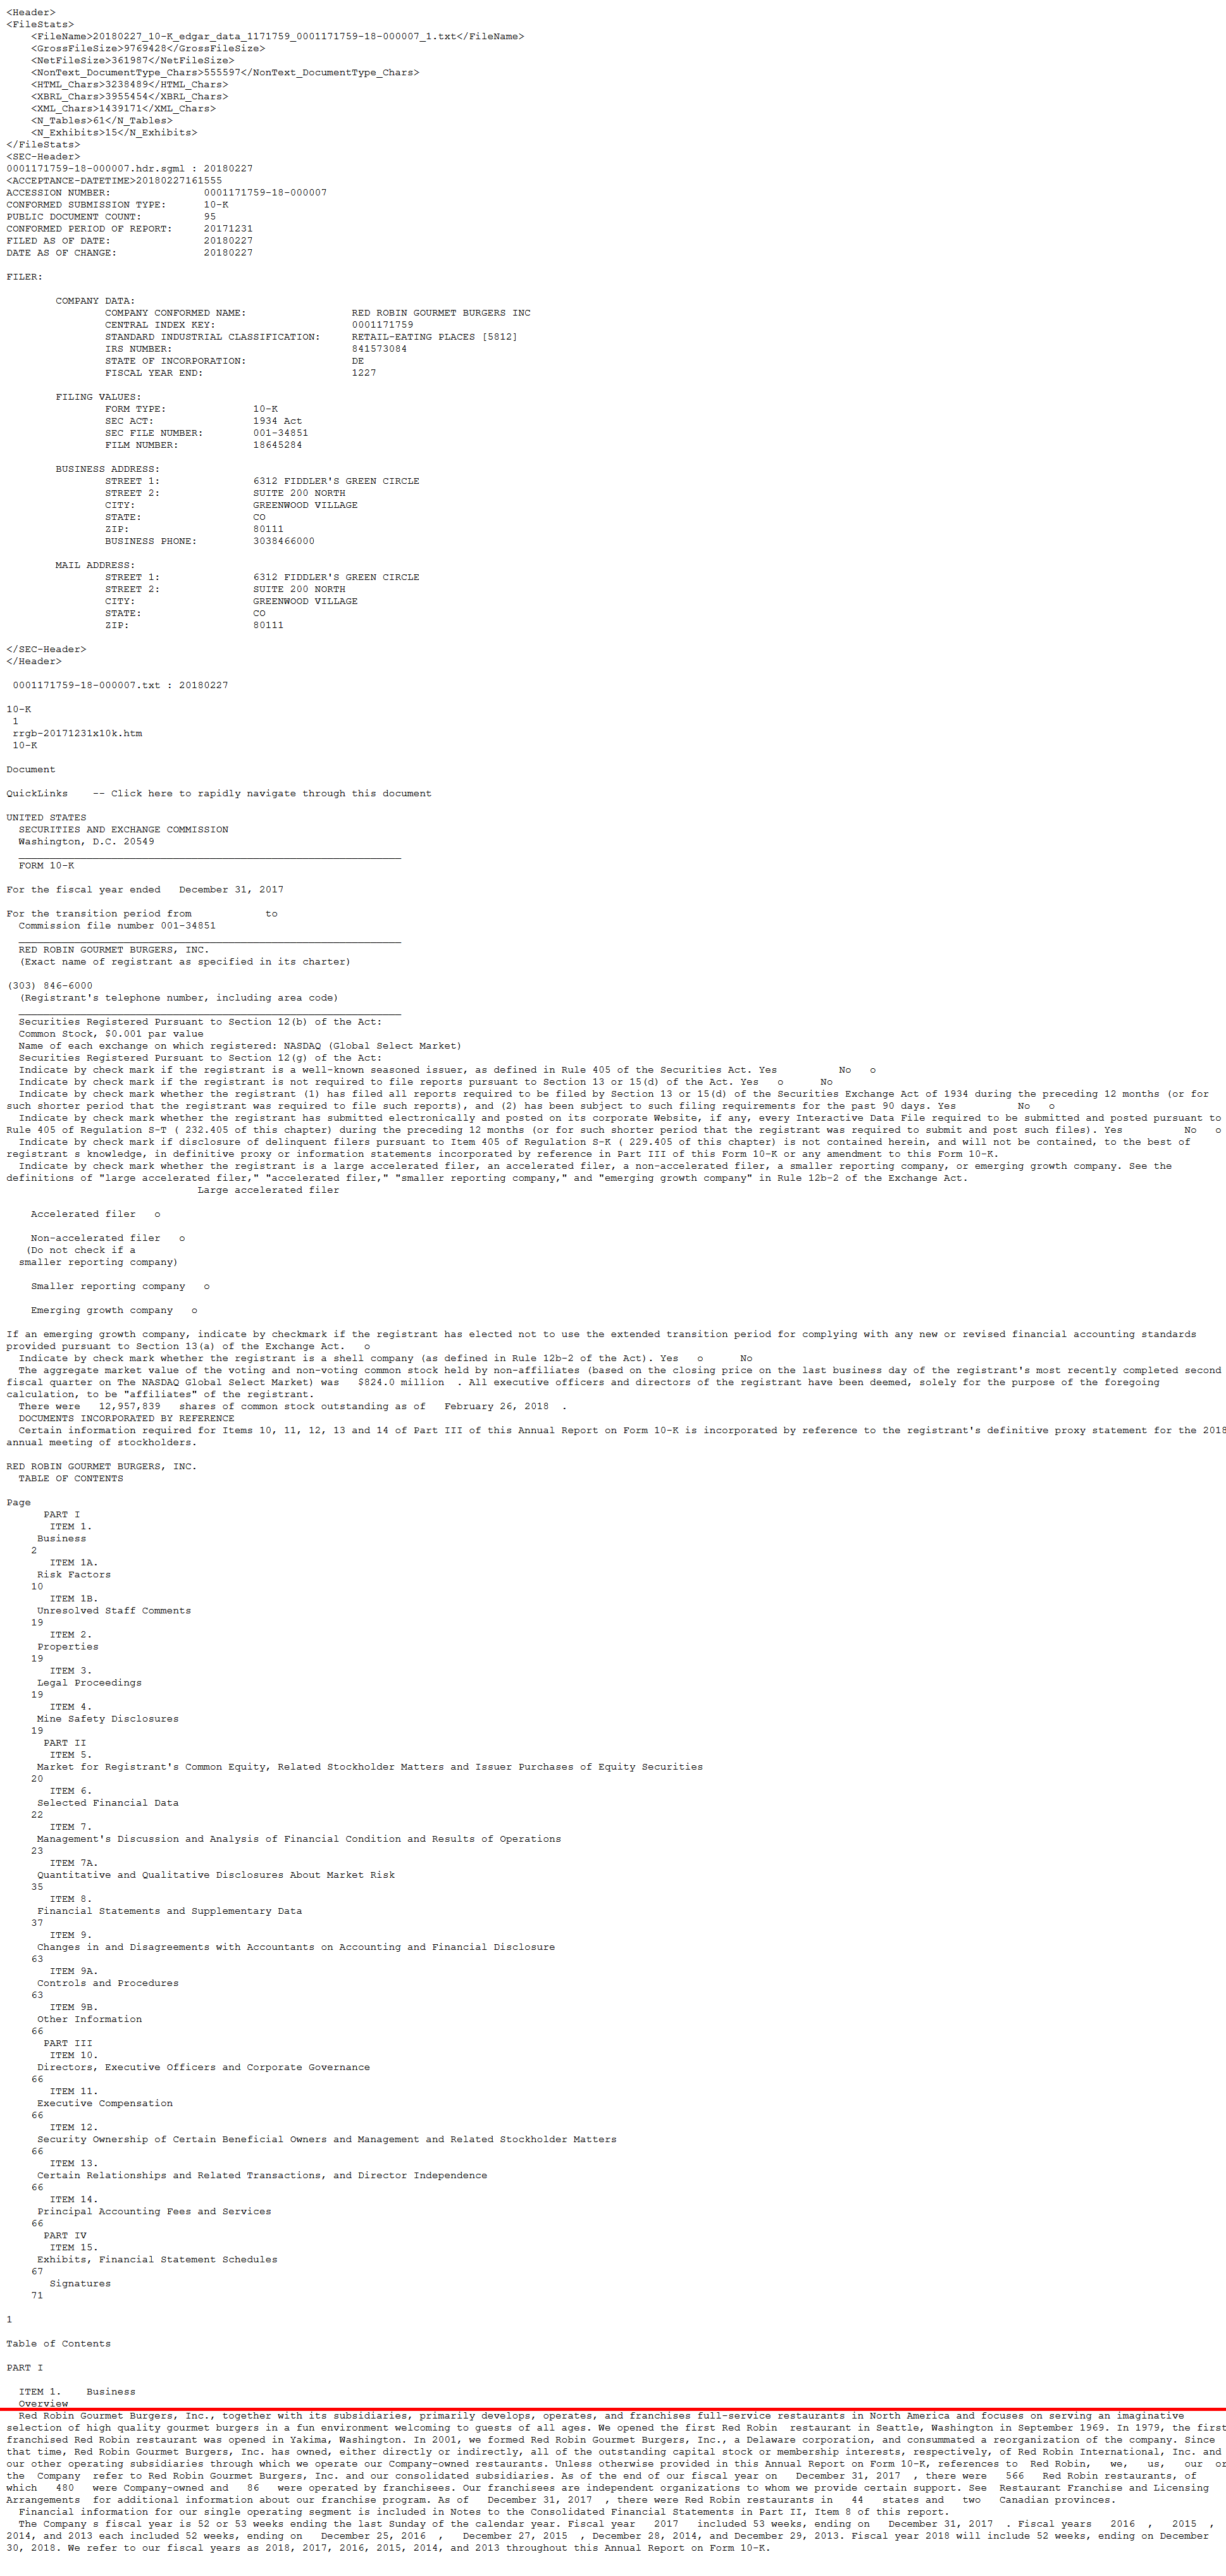
\includegraphics[width=0.6\textwidth]{figures/10-K_Start.png}
%     \caption{The beginning of a Form 10-K as it is loaded from the \ac{SRAF}.}
%     \label{figure:10k_start}
% \end{figure}
\FloatBarrier
\lstinputlisting[caption={The beginning of a Form 10-K as it is loaded from the \ac{SRAF}.}, label={listing:10k_start}]{listings/form_10k.txt}
Listing \ref{listing:10k_start} shows the beginning of a Form 10-K report as it is loaded from the \ac{SRAF}.
It can be seen, that this part of the file consists of the header data and generic text from the Form 10-K and can therefore be removed.
The table of contents, which follows after the text in listing \ref{listing:10k_start}, can also be removed.
This parsing however, was no trivial task:
Even though the Form 10-K and Form 10-Q are highly standardized, there are differences in detail between reports.
These range from different usage of capitalization, over different formats of numerations like "I-1", "Part I. Item 1." or "Items 1. and 2. Business and Properties", up to a different order of the items.
That made it infeasible to create a regular expression, which reliably detects the table on contents and regulatory texts.
Therefore another approach was taken: The reports were first splitted into sentences with the \texttt{\_splitReportToSentences} function, which is described by the structogram in figure \ref{figure:structogram_splitReportToSentences}.
\begin{figure}[h]
    \centering
    \includegraphics[width=1\textwidth]{figures/structogram_splitReportToSentences.png}
    \caption{High-level structogram of the \texttt{\_splitReportToSentences} function.}
    \label{figure:structogram_splitReportToSentences}
\end{figure}
This function is called for every report and uses the \textit{sentencizer} from the Python package spaCy to split the report into sentences.
It was interesting how long some of the resulting sentences were.
Bar chart \ref{figure:words_distribution} shows the distribution of different words per sentences.
\begin{figure}[h]
    \centering
    \includegraphics[width=0.6\textwidth]{figures/charts/words_distribution.png}
    \caption{Distribution of words per sentences.}
    \label{figure:words_distribution}
\end{figure}
It can be observed, that there is a huge number of sentences with less than 8 and some sentences with more than 95 words per sentence.
What the diagram does not show is the distribution for sentences with more than 200 words.
They account for 0.2\% of all sentences, with the longest sentence having 3905 words.
Sentences with less than 8 words are mostly headlines like "Item 2." or "Financial Statements and Supplementary Data Note 12.", sentences with more than 95 words appeared to be mostly regulatory texts.
Therefore these sentences were removed from the reports.
Some examples of these long sequences are given in appendix \ref{app:removed_sequences}.
Since the whole parsing process takes two seconds per report on average, the Python multiprocessing package was used to optimize the parsing for multiple \acs{CPU}s.
Therefore the parsing of the 27561 reports took about four hours on an Amazon EC2 instance with four v\acs{CPU}'s and 61 GB of memory.
After this parsing is finished the resulting files are added to an index file with the company's \ac{CIK}, stock ticker symbol, filing date, form type and the file path.

The second step covers the labeling of the reports as \textit{positive} or \textit{negative}.
For that another script runs through the index file again and retrieves the price information from the database using the script in listing \ref{py:get_prices}.
\lstinputlisting[language=Python,caption={Extract from the script that labels the reports},captionpos=b, label={py:get_prices}]{listings/get_prices.py}
The highest price change of stocks happens within two days after the release of a business report \cite{Feldman2010}, therefore the script retrieves three records from the database, which also includes the day of the report release itself.
The change ratio \textit{CR} on the date \textit{d} of a company with the ticker symbol \textit{t} is then computed as following:
\begin{equation}
    CR_{d,t} = \frac{p_{close, d + 2, t} - p_{open, d, t}}{p_{open, d, t}}
\end{equation}
Whereby $p_{open, d, t}$ is the opening stock price on the day of the report release and $p_{close, d + 2, t}$ is the closing price two days after the report has been released.
If the resulting change ratio is negative the report is labeled as \textit{negative} else it is labeled as \textit{positive}.
\begin{equation}
    CN(CR_{d,t}) = \begin{cases}
        positive & \text{for } CR_{d,t} \geq 0 \\
        negative & \text{for } CR_{d,t} < 0
    \end{cases}
\end{equation}
The resulting \ac{CSV} file has 24609 entries and each of these entries references one parsed report file.

Figure \ref{figure:data_flowchart} summarizes the steps described in this chapter.
\begin{figure}[h]
    \centering
    \includegraphics[width=0.6\textwidth]{figures/Flowchart_Data.png}
    \caption{The steps until the data is combined into one dataset.}
    \label{figure:data_flowchart}
\end{figure}
